\chapter{Grundlagen der Differenzialrechnung}
\section{Ableitung und Ableitungsregeln}

Gegeben ist $f$ auf $[a;b]$ 

\begin{tikzpicture}
\begin{axis}[clip=false, 
    xmin=0, xmax=4, ymin=0, ymax=10,
    axis lines = middle, 
    xlabel=$x$, ylabel=$y$,
    xtick={0,1,2,3,4}, xticklabels={0,a, ,b},
    ytick={0,2,4,6,8,10}, yticklabels={0,$f(a)$, $f(b)$}, grid = major]
\addplot[color=black, samples=50, domain=0.5:4]{0.5*(x-1)^2+2}node[right, pos = 0.8]{$G_f$};
\addplot[color=red, domain= 0.5:3.5]{x+1};
\draw [red, fill=yellow]  (1,2) node[thick, cross, red] {} node[below] {$P$};
\draw [red, fill=yellow]  (3,4) node[thick, cross, red] {} node[below] {$Q$};
\end{axis}
\end{tikzpicture}

$$\frac{f(b)-f(a)}{b-a}$$
heißt Differenzenqoutint von $f$ in $[a;b]$. Der Differenzenqoutient ist die Steigung m der Geraden durch $P(a|f(a))$ und $Q(b|f(b))$\footnotemark{}.

\flushbottom\footnotetext{genannt Sekantensteigung oder auch mittlere Änderungsrate}

\begin{tikzpicture}
\begin{axis}[clip=false, 
    xmin=0, xmax=4, ymin=0, ymax=10,
    axis lines = middle, 
    xlabel=$x$, ylabel=$y$,
    xtick={0,1,2,3,4}, xticklabels={0,$x_0$, ,$x_0+h$},
    ytick={0,2,4,6,8,10}, yticklabels={0,$f(x_0)$, $f(x_0+h)$}, grid = major]
\addplot[color=black, samples=50, domain=0.5:4]{0.5*(x-1)^2+2}node[right, pos = 0.8]{$G_f$};
\addplot[color=red, domain= 0.5:3.5]{x+1};
\draw [red, fill=yellow]  (1,2) node[thick, cross, red] {} node[below] {$P$};
\draw [red, fill=yellow]  (3,4) node[thick, cross, red] {} node[below] {$Q$};
\end{axis}
\end{tikzpicture}

Falls sich der Differenzenquotient $\frac{f(x_{0}+h)-f(x_{0})}{h}$ für $h \to 0$ einem festen Wert nähert, dann heißt dieser sogenannte Grenzwert Ableitung von $f$ an der Stelle $x_0$. $f$ ist an der Stelle $x_0$ differenzierbar. 

Geometrich: Tangentensteigung im Punkt $P(x_0|f(x_0))$.

Die Ableitung $f^{\prime}(x)$ ist also definiert durch:
$$f^{\prime}(x)=\lim_{h\to 0} \frac{f(x_{0}+h)-f(x_{0})}{h}$$
Eine Funktion, die jeder Stelle x die Ableitung $f^{\prime}(x)$ an dieser stelle zuordnet, heißt Ableitungsfunktion $f^{\prime}(x)$.

\noindent\rule{\textwidth}{1pt}

\textit{Beispiele:}

(1) S.12 Nr. 1 b)
\begin{equation*}
\begin{gathered}
    f(t)  = -4\sqrt{t}-3t \\
    = -4t^{\frac{1}{2}}-3t \\
    f^{\prime}(t)  = -2t^{-\frac{1}{2}}-3 \\
    f^{\prime\prime}(t)  = t^{-\frac{3}{2}} = \frac{1}{\sqrt{t^3}}
\end{gathered}
\end{equation*}
\begin{align*}
    D_f & = \mathbb{R}_0^+ = [0;\infty[ \ = [0;\infty) \text{\footnotemark}\\
    D_{f^\prime} & = \mathbb{R}^+ = \ ]0;\infty[ \\
    D_{f^{\prime\prime}} & = \mathbb{R}^+
\end{align*}
\footnotetext{alte Schreibweise}

e)
\begin{equation*}
    \begin{gathered}
        f(x)  = -\cos(x) + \frac{1}{x^2} = -\cos(x)+x^{-2} \\
    f^{\prime}(x)  = \sin(x) -2x^{-3} \\
    f^{\prime\prime}(x)  = \cos(x)+6x^{-4}
    \end{gathered}
\end{equation*}
\begin{align*}
    D_f = \mathbb{R} \ \backslash \ \{0\} = D_{f^{\prime}} = D_{f^{\prime\prime}}
\end{align*}

(2) S. 12 Nr. 2 b)
\begin{equation*}
    \begin{gathered}
        f(t)  = \frac{6t^3-t^2}{2t} = \frac{2t(3t^2 - \frac{1}{2}t)}{2t} = 3t^2 - \frac{1}{2}t \\
        f^{\prime}(x)  = 6t - \frac{1}{2}
    \end{gathered}
\end{equation*}
\begin{align*}
    D_f & = \mathbb{R} \ \backslash \ \{0\}  \\
    D_{f^{\prime}} & = \mathbb{R}
\end{align*}

e)
\begin{equation*}
    \begin{gathered}
        f(s)  = (2s-4)\cdot(4-s) = 8s-2s^2-16+4s = -2s^2 + 8s -16\\
        f^{\prime}(s)  = -4s +8 
    \end{gathered}
\end{equation*}
\begin{align*}
    D_f = \mathbb{R} = D_{f^{\prime}}
\end{align*}

\section{Verketten von Funktionen}
Vorüberlegung:

$u(x)= x^2 \ , \ v(x) = x + 2$

Summen von $u$ und $v$:
$$u(x)+v(x) = x^2 +x+2 = (u + v)(x)$$

Differenz von $u$ und $v$:
$$u(x)-v(x)=x^2-x-2 = (u-v)(x)$$

Produkt von $u$ und $v$:
$$u(x) \cdot v(x) = x^3+ 2x = (u \cdot v)(x)$$

Quotient von $u$ und $v$:
$$\frac{u(x)}{v(x)} = \frac{x^2}{x+2}$$

\begin{definition}
Unter der Verkettung der beiden Funktionen $u$ und $v$ versteht man die Funktion $f$ mit
$$f(x)=u(v(x))$$
\end{definition}

$u$ heißt äußere Funktion, $v$ heißt innere Funktion der Verkettung. Schreibweise: $f = u \circ v$ (lies: \glqq $u$ nach $v$\grqq{} oder  \glqq $u$ verkettet $v$\grqq{} ).

\noindent\rule{\textwidth}{1pt}

\textit{Beispiele:}

$u(x) = x^2 \ , \ v(x) = x + 2$

$f(x) = u(v(x)) = (x+2)^2 \\ g(x) = v(u(x)) = x^2 + 2$

\textbf{Beachte:} Die Verkettung zweier Funktionen ist i. a. nicht kommutativ d. h. $u \circ v \neq v \circ u$.

\section{Kettenregel}

\begin{satz}
    Ist $f = u \circ v$ eine Verkettung zweier differenzirbarer Funktionen $u$ und $v$ so ist $f$ auch differenzierbar und es gilt:

$$f^{\prime}(x) = u^{\prime}(v(x)) \cdot v^{\prime}(x)$$
\end{satz}

kurz: \glqq Ableitung der Gesamtfunktion ist gleich äußere Ableitung mal innere Abeitung.\grqq{}

\noindent\rule{\textwidth}{1pt}

\textit{Beispiele:}

(1)
\begin{equation*}
    \begin{gathered}
        f(x)  = (5-3x)^4 \\
        f^{\prime}(x)  = 4(5-3x)^3 \cdot (-3) = -12(5-3x)^3
    \end{gathered}
\end{equation*}

(2)
\begin{equation*}
    \begin{gathered}
        f(x)  = \sqrt{x^2 + 1} = (x^2 + 1)^\frac{1}{2} \\
        f^{\prime}(x)  = \frac{2x}{2\sqrt{x^2 + 1}} = \frac{x}{\sqrt{x^2 + 1}}
    \end{gathered}
\end{equation*}

(3)
\begin{equation*}
    \begin{gathered}
        f(x)  = \frac{3}{2x^2 - 1} = 3(2x^2 - 1)^{-1} \\
        f^{\prime}(x)  = \frac{-12x}{(2x^2 - 1)^2}
    \end{gathered}
\end{equation*}

(4)
\begin{equation*}
    \begin{gathered}
        f(x)  = 3\sin(2x^3) \\
        f^{\prime}(x)  = 18x^2\cos(2x^3)
    \end{gathered}
\end{equation*}

\section{Produktregel}

\begin{satz}
Sind die Funktionen $u$ und $v$ differenzierbar, so ist auch die Funktion $f$ mit $f = u \cdot v$ differenzierbar, und es gilt \footnote{sehr selten: $f(x) = u\cdot v\cdot w \quad , \quad f^\prime(x) = u^\prime \cdot v \cdot w + u \cdot v^\prime \cdot w + u \cdot v \cdot w^\prime$}:
$$f^\prime(x) = u^\prime(x) \cdot v(x) + u(x) \cdot v^\prime(x)$$
\end{satz}

\noindent\rule{\textwidth}{1pt}

\textit{Beispiele:}

(1) 
\begin{equation*}
    \begin{gathered}
    f(x) = x^2 \sin(x) \\
    f^\prime(x) = 2x \sin(x) + x^2 \cos(x)
    \end{gathered}
\end{equation*}

(2) 
\begin{equation*}
    \begin{gathered}
     f(x)  = \sqrt{x}(4x + 1) \\
     f^\prime(x)  = \frac{4x + 1}{2\sqrt{x}} + 4 \sqrt{x}    
    \end{gathered}
\end{equation*}

(3) 
\begin{equation*}
    \begin{gathered}
     f(x)  = (2x - 3) \cos(4x) \\
     f^\prime(x)  = 2\cos(4x)-4(2x-3)\sin(4x)    
    \end{gathered}
\end{equation*}

\ \\
\ \\
\ \\
\ \\
\ \\

(4) Der Graph von $f$ hat im Punkt $P(0|1)$ eine waagrechte Tangente. Untersuchen Sie, ob dies auch für den Graph der Funktion $g$ mit $g(x) = f(x) \cdot \cos(x)$ gilt.\\

$G_f: P(0|1) \in G_f$ mit waagrechter Tangente $\Rightarrow f(0) = 1$ und $f^\prime(0) = 0$ \\
zu zeigen: $g(0) = 1$ und $g^\prime(0) = 0$
\begin{equation*}
    \begin{gathered}
        g(x) = f(x) \cdot \cos(x) \\
        g^\prime(x) = f^\prime(x) \cdot \cos(x) - f(x) \cdot \sin(x)
    \end{gathered}
\end{equation*} 
Also:
\begin{equation*}
    \begin{gathered}
        g(0) = f(0) \cdot \cos(0) = 1 \cdot 1 = 1 \Rightarrow P(0|1) \in G_g \tag{1} \label{1} \\
    \end{gathered}
\end{equation*}
\begin{equation*}
    \begin{gathered}
        g^\prime(0) = f^\prime(0) \cdot \cos(0) - f(0) \cdot \sin(0) = 0 \Rightarrow \text{$G_g$ hat bei $P$ eine waagrechte Tangente} \tag{2} \label{2}
    \end{gathered}
\end{equation*}

Aus \eqref{1} und \eqref{2} folgt die Behauptung.

\section{Monotonie und Krümmung}
Wiederholung:

Gegeben ist der Graph $G_f$:

\begin{tikzpicture}
\draw[step=1.0,lightgray,very thin] (0,0) grid (7.2,5.8);
\begin{axis}[clip=true, 
    xmin=0, xmax=8, ymin=0, ymax=10,
    axis lines = middle, 
    xlabel=$x$, ylabel=$y$,
    xtick={3.92,6.06, 6.76}, xticklabels={$x_1$, $x_2$, $x_3$},
    ytick={6.22, 7.26, 8.61}, yticklabels={$f(x_1)$,$f(x_3)$, $f(x_2)$}]
\addplot[color=black, samples=100, domain=0.7:7.5]{-0.05*(x-2)^2*3*(0.8*(x-6)^2-0.25)+8}node[right, pos = 0.8]{$G_f$};
\draw [red, fill=yellow]  (3.92,6.22) node[thick, cross, red] {} node[below] {$x_1$};
\draw [red, fill=yellow]  (6.08,8.61) node[thick, cross, red] {} node[below] {$x_2$};
\draw [red, fill=yellow]  (6.76, 7.26) node[thick, cross, red] {} node[right] {$x_3$};
\end{axis}
\end{tikzpicture}
\begin{definition}
    Wenn für alle $x_1$, $x_2$ mit $x_1 < x_2$ auf einem Intervall $I$ gilt:
    
    $f(x_1) < f(x_2)$, dann heißt $f$ streng monton wachsend auf I

    $f(x_1) > f(x_2)$, dann heißt $f$ streng monton fallend auf I \footnote{Beachte: die Ränder von Monotonierintervallen kann man zu beiden Monotonieintervallen dazunehmen. Intervall, in dem die Funktion $f$ \\ (1) streng monoton wachsend ist: $[x_1;x_2]$ \\(2) strend monoton fallend ist: $[x_2;x_3]$} \\
\end{definition}
\begin{satz}[Monotoniesatz]
    Die Funktion $f$ sei im Intervall $I$ differenzierbar. Wenn für alle $x \in I$ gilt:

    $f^\prime(x) > 0$, dann ist die Funktion $f$ streng monoton wachsend auf $I$. 
    
    $f^\prime(x) < 0$, dann ist die Funktion $f$ streng monoton fallend auf $I$. \footnote{Die Umkehrung des Monotoniesatzes gilt nicht.} \\
\end{satz}

\begin{figure}[h]
    \centering
    \captionsetup[subfigure]{oneside,margin={-1cm,0cm}}
    \begin{subfigure}[h]{0.49\textwidth}
        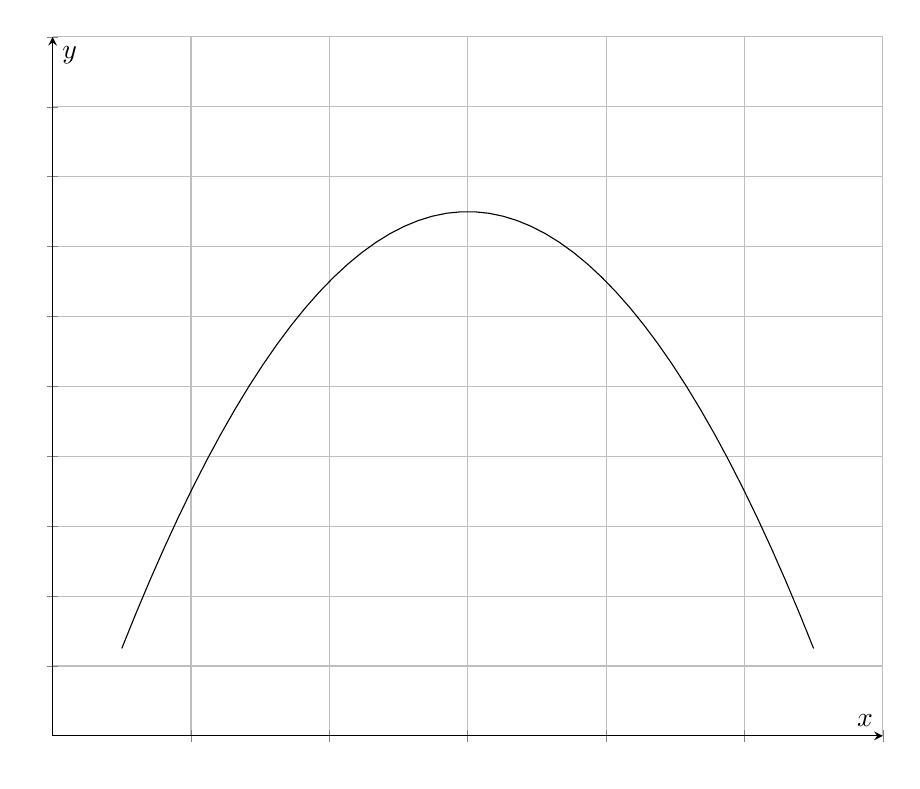
\begin{tikzpicture}
        \begin{axis}[clip=false, 
            xmin=0, xmax=6, ymin=0, ymax=10,
            axis lines = middle, 
            xlabel=$x$, ylabel=$y$,
            xtick={}, xticklabels={},
            ytick={}, yticklabels={},
            width=\linewidth, grid = major]
        \addplot[color=black, samples=50, domain=0.5:5.5]{-(x-3)^2 +7.5};
        \end{axis}
        \end{tikzpicture} 
    \caption*{Rechtskurve}
    \end{subfigure}
    \begin{subfigure}[h]{0.49\textwidth}
        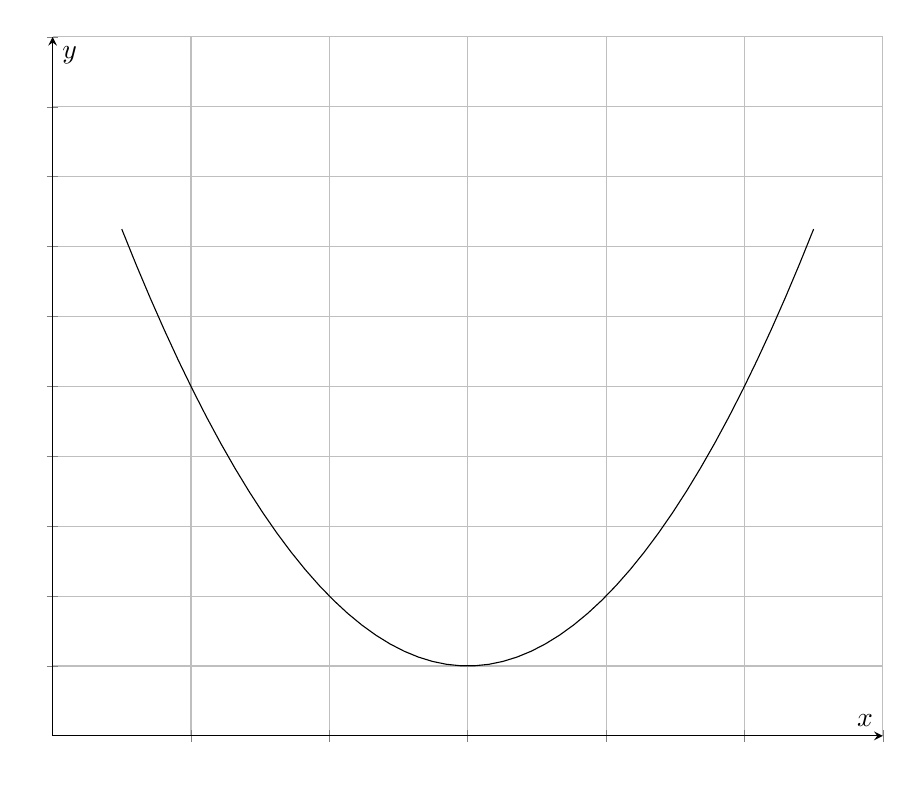
\begin{tikzpicture}
        \begin{axis}[clip=false, 
            xmin=0, xmax=6, ymin=0, ymax=10,
            axis lines = middle, 
            xlabel=$x$, ylabel=$y$,
            xtick={}, xticklabels={},
            ytick={}, yticklabels={},
            width=\linewidth, grid = major]
        \addplot[color=black, samples=50, domain=0.5:5.5]{(x-3)^2 +1};
        \end{axis}
        \end{tikzpicture} 
    \caption*{Linkskurve}
    \end{subfigure}
    \label{fig:enter-label}
\end{figure}

\begin{tabularx}{\textwidth} { 
  | >{\raggedright\arraybackslash}X 
  | >{\centering\arraybackslash}X 
  | >{\centering\arraybackslash}X | }
 \hline
  & Rechtskurve & Linkskurve \\
 \hline
 $f^\prime(x)$ ist streng monoton  & fallend & steigend  \\
 \hline
 $f^{\prime\prime}(x)$ & < 0 & > 0 \\
\hline
\end{tabularx}

\noindent\rule{\textwidth}{1pt}

\textit{Beispiel: Bestimmung des Krümmungsverhaltens}

\begin{equation*}
    \begin{gathered}
        f(x) = \frac{1}{4}x^4-\frac{4}{3}x^3+2x^2+2 \\
        f^\prime(x) = x^3-4x^2+4x \\
        f^{\prime\prime}(x) = 3x^2-8x + 4
    \end{gathered}
\end{equation*}

\begin{equation*}
    \begin{gathered}
        f^{\prime\prime}(x) = 0 \\
        0 = 3x^2-8x + 4
    \end{gathered}
\end{equation*}

Mitternachtsformel:

\begin{equation*}
    \begin{gathered}
        x_{1,2}=\frac{8\pm\sqrt{(-8)^2-4\cdot3\cdot4}}{2\cdot3} \Rightarrow x_1 = 2 \ , \ x_2 = \frac{2}{3}
    \end{gathered}
\end{equation*}

Das heißt: 

\begin{tabularx}{\textwidth} { 
  | >{\raggedright\arraybackslash}X 
  | >{\centering\arraybackslash}X
  | >{\centering\arraybackslash}X
  | >{\centering\arraybackslash}X
  | >{\centering\arraybackslash}X
  | >{\centering\arraybackslash}X | }
 \hline
  & $x < \frac{2}{3}$ & $x = \frac{2}{3}$ & $\frac{2}{3} < x < 2$ & $x = 2$ & $x > 2$ \\
 \hline
 $f^{\prime\prime}(x)$  & $>0$ & $0$ & $<0$ & $0$ & $>0$  \\
 \hline
 $f^{\prime}(x)$ & streng monoton wachsend & - & streng monoton fallend & - & streng monoton wachsend \\
 \hline
 $G_f$ & Linkskurve & - & Rechtskurve & - & Linkskurve \\
\hline
\end{tabularx}

\section{Extrem- und Wendepunkte}
\textbf{Flussdiagramm:} Bestimmung der lokalen Extrema einer Funktion $f$

Die Funktion $f$ sei zweimal differenzierbar.\\

\begin{tikzpicture}[node distance=2cm, text width= 4cm]
    \node (pro1) [process, text width=4cm] {notwendige Bedingung $f^\prime(x) = 0$};
    \node (pro2a) [process, text width=4cm, below of=pro1] {es existiert \\ eine Lösung};
    \node (pro2b) [process, text width=4cm, below of=pro1, xshift = 8cm] {es existiert keine Lösung};
    \node (pro3a) [process, text width=4cm, below of=pro2a] {hinreichende Bedingung $f^\prime(x) = 0 \land f^{\prime\prime}(x) \neq 0$};
    \node (pro3b) [process, text width=4cm, below of=pro2b] {keine Extrema};
    \node (pro4a) [process, text width=4cm, below of=pro3a, xshift = 1cm, yshift= -0.5cm] {$f^{\prime\prime}(x) < 0$ \\ x ist Maximumstelle};
    \node (pro4b) [process, text width=4cm, below of=pro3a, xshift = -4cm, yshift= -0.5cm] {$f^{\prime\prime}(x) > 0$ \\ x ist Minimumstelle};
    \node (pro4c) [process, text width=4cm, below of=pro3a, xshift= 7cm,  yshift= -0.5cm] {$f^{\prime\prime}(x) = 0$};
    \node (pro5) [process, text width=4cm, below of=pro4c] {VZW-Kriterium\footnotemark \\ von $f^\prime$ in der Umgebung von $x$};
    \node (pro6a) [process, text width=4cm, below of=pro5, xshift= -2cm, yshift= -0.5cm] {VZW von \\
                                                        $-$ nach $+$ \\
                                                        $x$ ist Minimumstelle};
    \node (pro6b) [process, text width=4cm, left of=pro6a, xshift = -2.5cm] {VZW von \\
                                                        $+$ nach $-$ \\
                                                        $x$ ist Maximumstelle};
    \node (pro6c) [process, text width=4cm, right of=pro6a, xshift = 2.5cm] {kein VZW \\
                                                        \quad \newline
                                                        keine Extrema};
    \node (pro7) [process, text width=4cm, below of=pro4b, yshift = -4.5cm] {Berechne $f(x)$};

    \draw [arrow] (pro1) -- (pro2a);
    \draw [arrow] (pro1) -| (pro2b);
    \draw [arrow] (pro2a) -- (pro3a);
    \draw [arrow] (pro2b) -- (pro3b);
    \draw [arrow] (pro3a) -- (pro4a);
    \draw [arrow] (pro3a) -- (pro4b);
    \draw [arrow] (pro3a) -- (pro4c);
    \draw [arrow] (pro4c) -- (pro5);
    \draw [arrow] (pro5) -- (pro6a);
    \draw [arrow] (pro5) -- (pro6b);
    \draw [arrow] (pro5) -- (pro6c);
    \draw [arrow] (pro4a) -- (pro7);
    \draw [arrow] (pro4b) -- (pro7);
    \draw [arrow] (pro6a) |- (pro7);
    \draw [arrow] (pro6b) -- (pro7);
\end{tikzpicture}

\footnotetext{VZW = Vorzeichenwechsel}

\textit{Beispiel:}

\begin{equation*}
    \begin{gathered}
        f(x) = -\frac{1}{4}x^4 + \frac{1}{3}x^3 + 1
    \end{gathered}
\end{equation*}

\textbf{Extremepunkte:}

\begin{equation*}
    \begin{gathered}
        f^\prime(x)=-x^3+x^2 \\
        f^{\prime\prime}(x)=-3x^2 + 2x
    \end{gathered}
\end{equation*}

notwendige Bedingung: $f^\prime(x) = 0$

\begin{equation*}
    \begin{gathered}
        0 = -x^3+x^2 \\
        0 = x^2  (-x+1) \\
        \Rightarrow \text{Satz vom Nullprodukt: } x_1 = 0, \ x_2 = 1
    \end{gathered}
\end{equation*}

hinreichende Bedingung: $f^\prime(x) = 0 \land f^{\prime\prime}(x)\neq0$

\begin{equation*}
    \begin{gathered}
        f^{\prime\prime}(0)=0 \Rightarrow \text{keine Aussage möglich}
    \end{gathered}
\end{equation*}

VZW von $f^\prime$ in der Umgebung von $x_1 = 0$:
\begin{equation*}
    \begin{gathered}
        \text{für } x < 0 \text{ gilt: } f^\prime(x)=x^2(-x+1) > 0 \\
        \text{für } x > 0 \text{ gilt: } f^\prime(x)=x^2(-x+1) > 0 \\
        \Rightarrow f \text{ hat keinen VZW an der Stelle } x_1 = 0 \text{ , also ist } x_1 \text{ auch keine Extremstelle.}
    \end{gathered}
\end{equation*}

\begin{equation*}
    \begin{gathered}
        f^{\prime\prime}(1) = -1 \neq 0 \\
        f^{\prime\prime}(1) < 0 \Rightarrow \text{Maximumstelle}
    \end{gathered}
\end{equation*}

\begin{equation*}
    \begin{gathered}
        f(1) = \frac{13}{12} \ \Rightarrow \text{Hochpunkt } H\left(1 \ \middle| \ \frac{13}{12}\right)
    \end{gathered}
\end{equation*}

\ \\
\ \\
\ \\
\ \\
\ \\
\ \\
\ \\

\textbf{Wendepunkte:}

\begin{equation*}
    \begin{gathered}
        f^{\prime\prime}(x)=-3x^2 + 2x \\
        f^{\prime\prime\prime}(x) = -6x + 2
    \end{gathered}
\end{equation*}

notwendige Bedingung: $f^{\prime\prime}(x)=0$

\begin{equation*}
    \begin{gathered}
        0 = -3x^2 + 2x \\
        0 = -x(3x-2) \\
        \Rightarrow \text{Satz vom Nullprodukt: } x_1 = 0, \ x_2 = \frac{2}{3}
    \end{gathered}
\end{equation*}

hinreichende Bedingung: $f^{\prime\prime}(x)=0 \land f^{\prime\prime\prime}(x) \neq 0$

\begin{equation*}
    \begin{gathered}
        f^{\prime\prime\prime}(0)= 2 \neq 0 \Rightarrow \text{Wendestelle} \\
        f^{\prime\prime\prime}\left(\frac{2}{3}\right)= -2 \neq 0 \Rightarrow \text{Wendestelle}
    \end{gathered}
\end{equation*}

Damit:

\begin{equation*}
    \begin{gathered}
        W_1(0 \ | \ f(0)) \text{, also: } W_1(0 \ | \ 1) \\
        W_2\left(\frac{2}{3} \ \middle| \ f\left(\frac{2}{3}\right)\right) \text{, also: } W_2\left(\frac{2}{3} \ \middle| \ \frac{85}{81}\right) \\
    \end{gathered}
\end{equation*}

\textbf{Anmerkung:}

Bei $W_1$ handelt es sich um einen Sattelpunkt\footnote{= Wendepunkt mit waagrechter Tangente}.


\section{Tangente und Normale}

\begin{definition}
    Die Gerade, die senkrecht zu einer Tangente verläuft heißt Normale. Sie hat die Steigung 
    $$-\frac{1}{m_t} = -\frac{1}{f^\prime(x)} \qquad \text{, falls } f^\prime(x) \neq 0 \text{ ist.}$$
\end{definition}

\pagebreak

\textit{Beispiel:}

Gesucht: Gleichung der Normalen an $G_f$ im Punkt $P\left(2\middle|\frac{1}{2}\right)$.

\begin{equation*}
    \begin{gathered}
        f(x) = \frac{1}{x} \\
        f^\prime(x) = -\frac{1}{x^2} \\
        f^\prime(2) = -\frac{1}{2^2} = -\frac{1}{4} = m_t
    \end{gathered}
\end{equation*}

Also:

\begin{equation*}
    \begin{gathered}
        m_n = 4 \Rightarrow n(x) = 4x + c \\
        P \text{ in } n(x): \ \frac{1}{2} = 4\cdot2 + c \Leftrightarrow c = -\frac{15}{2} \\
        n(x) = 4x - \frac{15}{2}
    \end{gathered}
\end{equation*}

\section{Extremwertprobleme mit Nebenbedingung}
\subsection{Extremwertproblem: Volumenminimierung, Oberflächenminimierung, etc.}

\textit{Beispiel: Getränkedose}

Eine handelsübliche (zylindrische) Cola-Dose enthält 0,33 l des Getränks, insgesamt beträgt das Volumen 0,35 l. Ein Hersteller möchte aus Umweltschutz- und Kostengründen seine Dose so konstuieren, dass er so wenig Verpackungsmaterial (Aluminium) wie möglich benötigt.

Bestimme wie groß dann der Radius und die Höhe der \glqq optimalen\grqq{} Dose sein müssen.

Ziel: Minimierung der Dosenoberfläche 

\begin{equation*}
    A = 2\pi \cdot r^2 + U \cdot h \tag{1}\label{3}
\end{equation*}
\begin{equation*}
    V = G \cdot h = \pi r^2 \cdot h = 0,35 \tag{2}\label{4}
\end{equation*}

Auflösen der Nebenbedingung \eqref{4} nach $h$:

\begin{equation*}
    h = \frac{0,35}{\pi r^2} \label{5}\tag{3}
\end{equation*}

\eqref{5} in \eqref{3} einsetzen: $$A(r) = 2\pi r^2 + 2\pi r\cdot\frac{0,35}{\pi r^2} = 2\pi r^2 + \frac{0,7}{r} \qquad \qquad \text{ ,mit } D_A = \ ]0;\infty[ \ = \mathbb{R}^+ $$

\begin{equation*}
    \begin{gathered}
        A(r) = 2\pi r^2 + 0,7r^{-1} \\
        A^\prime(r) = 4\pi r - 0,7^{-2} \\
        A^{\prime\prime}(r) = 4\pi + 1,4r^{-3}
    \end{gathered}
\end{equation*}

notwendige Bedingung: $A^\prime(r) = 0$

\begin{equation*}
    \begin{gathered}
        0 = 4\pi r - 0,7^{-2} \\
        0 = 4\pi r^3 - 0,7 \\
        0,7 = 4\pi r^3 \\
        r = \sqrt[3]{\frac{0,7}{4\pi}}
    \end{gathered}
\end{equation*}

hinreichende Bedingung: $A^\prime(r) = 0 \land A^{\prime\prime}(r) \neq 0$

\begin{equation*}
    \begin{gathered}
        A^{\prime\prime}\left(\sqrt[3]{\frac{0,7}{4\pi}}\right) \approx 12\pi > 0 \Rightarrow \text{ lokale Minimumstelle} \\
        A\left(\sqrt[3]{\frac{0,7}{4\pi}}\right) \approx 2,749
    \end{gathered}
\end{equation*}

Randwertbetrachtung: 

$\text{für }  r \to 0  \text{ gilt: }  \underbrace{2\pi r^2}_{\to 0} + \underbrace{\frac{0,7}{r}}_{\to \infty} \to \infty \\
\text{für }  r \to \infty \text{ gilt: }  \underbrace{2\pi r^2}_{\to \infty} + \underbrace{\frac{0,7}{r}}_{\to 0} \to \infty$

$\Rightarrow$ keine weiteren Minima

Also: 

$r = \sqrt[3]{\frac{0,7}{4\pi}}$ in \eqref{5}: $ h \approx 0, 76 $

Die \glqq optimale\grqq{} Dose hat folglich eine Radius von ca. 0,38 cm und eine Höhe von ca. 0,76 cm.

\subsection{Extremwertproblem: Kleinster Abstand eines Punktes zu einem Graphen}

Hier soll der kleinste Abstand eines Punktes $P(a \ |  \ b)$ von dem Graph einer Funktion $f$ bestimmt werden. Dazu wird auf dem Graph ein belibiger Punkt $Q(u \ | \ f(u))$ ausgewählt und mit dem \textbf{Satz des Pythagoras} der Abstand zu $P(P_x \ |  \ P_y)$ berechnet.\\
Dieser Abstand ist die Zielfunktion $z(u)$ deren kleinster Wert zu bestimmen ist:
$$z(u) = \sqrt{(u-P_x)^2 + (f(u)-P_y)^2}$$
Die \textbf{Nebenbedingungen} sind hier die Seitenlängen $u - P_x$ und $f(u) - P_y$ des dargestellten Dreiecks.

\begin{tikzpicture}
\begin{axis}[clip=false, 
    xmin=-3, xmax=8.5, ymin=-2, ymax=5.5,
    axis lines = middle, 
    xlabel=$x$, ylabel=$y$,
    xtick={-2,-1,0,1,2,3,4,4.5,5,6,7,8}, xticklabels={-2,-1,0,1,$P_x$,3,4,$u$,5,6,7,8},
    ytick={-1,0,1,2,3,3.25,4,5}, yticklabels={-1,0,1,$P_y$, ,$f(u)$,4,5},
    width=16.5cm, height = 12cm]
    \addplot[thick, color=black, samples=50, domain=3.5:6.5]{(x-5)^2+3}node[right, pos = 0.9]{$G_f$};
    \draw (4.60,3.25) node[anchor= south west, fill=white] {$Q(u  | f(u))$};
    \draw (3.25,2.00) node[below] {$a=u - P_x$};
    \draw (2.60,2.35) node[above] {$z(u)$};
    \draw (4.50,2.50) node[right] {$b=f(u)-P_y$};
    \draw [dashed] (2,2) -- (2,0);
    \draw [dashed] (2,2) -- (0,2);
    \draw [dashed] (4.5,2) -- (4.5,0);
    \draw [dashed] (4.5,3.25) -- (0,3.25);

    \addplot[thick, mark=,black] coordinates {(4.5,3.25) (2,2) (4.5,2) (4.5,3.25)};
    
    \draw (4.50,3.25) node[thick, cross,red] {};
    \draw (2,2) node[thick, cross,red] {} node[anchor= north east] {$P(P_x | P_y)$};
    \draw (4.5,2) node[thick, cross,red] {};
\end{axis}

\end{tikzpicture}


\noindent\rule{\textwidth}{1pt}

\textit{Beispiel:}\\
Betrachtet werden die Funktion $f$ mit $f(x) = 0,5x^2 + 1$ und der Punkt $P(4 \ | \ 2)$. Bestimme den Punkt $Q$ auf dem Grapfen von $f$, der den kleinsten Abstand von $P$ hat. Gib den kleinsten Abstand an.

\pagebreak

(1) Ggf. eine Skizze erstellen nach dem oben gegebenen Schema. \\

\begin{tikzpicture}
\begin{axis}[clip=false, 
    xmin=-3.5, xmax=6.5, ymin=-0.5, ymax=4.5,
    axis lines = middle, 
    xlabel=$x$, ylabel=$y$,
    xtick={-3, -2,-1,0,1,2,3,4,5,6}, xticklabels={-3, -2,-1,0,1,$u$,3,4,5,6},
    ytick={0,1,2,3,4}, yticklabels={0,1,2,$f(u)$,4},
    width=11cm, height = 8cm]
    \addplot[thick, color=black, samples=50, domain=-2.5:2.5]{0.5*x^2 + 1}node[right, pos = 0.95]{$G_f$};

    \addplot[thick, mark=,black] coordinates {(2,3) (4,2) (2,2) (2,3)};

    \draw (2,3) node[anchor= south east] {$Q$};
    \draw (2,2.5) node[right] {$b$};
    \draw (3,2) node[below] {$a$};
    \draw (3.3,2.4) node[right] {$z$};

    \draw [dashed] (2,2) -- (2,0);
    \draw [dashed] (2,3) -- (0,3);
    
    \draw (2,3) node[thick, cross, red] {};
    \draw (2,2) node[thick, cross, red] {};
    \draw (4,2) node[thick, cross, red] {} node[right] {$P$};

\end{axis}
\end{tikzpicture}

(2) Beschreibe den formalen Zusammenhang der betrachteten Größen. Nutze dazu die Bezeichnungen aus deiner Skizze.\\
$z^2 = b^2 + a^2$ \newline

(3) Schreibe die Nebenbedingung auf. \\
$a = P_x -u \\ b = f(u) - P_y$ \newline

(4) Setze die Nebenbedingung ein und stelle die Zielfunktion auf. \\
$z^2 = (4-u)^2 + ((0,5u^2+1)-2)^2$ \\
Also: $$z(u) = \sqrt{(4-u)^2 + ((0,5u^2-1)^2} = \sqrt{16-8u+u^2+0,25u^4-u^2+1} $$
$$z(u) = \sqrt{0,25u^4 -8u +17}$$

(5) Leite die Zielfunktion ab und bestimme mögliche Extremstellen. \\
$$z^\prime(u) = \frac{u^3 -8}{2\sqrt{0,25u^4 -8u +17}}$$

notwendige Bedingung: $z^\prime(u) = 0$
\begin{equation*}
    \begin{aligned}
        0 & = \frac{u^3 -8}{2\sqrt{0,25u^4 -8u +17}} & \qquad & |\cdot 2\sqrt{0,25u^4 -8u +17} \\
        0 & = u^3 - 8 & \qquad & | +8 \\
        8 & = u^3 & & | \sqrt[3]{} \\
        u & = 2
    \end{aligned}
\end{equation*}

(6) Bestimme die Art der Extremstelle. \\

VZW-Kriterium: \\
für $u>2 \land u \to 2$ gilt: $z(u) < 0$ \\
für $u<2 \land u \to 2$ gilt: $z(u) > 0$ \\
$\Rightarrow$ VZW von $-$ nach $+ \Rightarrow u = 2$ ist Minimumstelle

(7) Bestimme die Koordinaten von Q.\\

Da $Q \in G_f$: $f(2) = 0,5\cdot2^2 +1 = 3$\\
Also: $Q(2 \ | \ 3)$

(8) Bestimme den kleinsten Abstand.\\

$z(2) = \sqrt{5} \approx 2,24$